\chapter{The noise spectrum}\label{ch:noise}

The \ui{Noise spectrum} panel on the Data page summarises how much energy the ground contained at each frequency during
the selected time, as a median curve with a band around it. It is the quickest way to judge a site, to compare day with
night, and to spot a new source of interference.

\section{Definition}
Start from the spectrogram grid $P[m,k]$ of Eq.~\eqref{eq:specdb} (columns $m$ are times, rows $k$ frequencies).
\begin{enumerate}
\item Drop every column that is entirely not-a-number, that is, every window touching a gap.
\item Drop the zero-frequency row.
\item For each frequency $f_k$ compute three \emph{percentiles} across the remaining columns:
  \[
    P_{10}[k],\qquad P_{50}[k]=\median_m P[m,k],\qquad P_{90}[k].
  \]
\end{enumerate}
The panel draws $P_{50}$ as a line and the range $P_{10}$--$P_{90}$ as a band on a logarithmic frequency axis.

Percentiles, and not the mean, are used because they are \emph{robust}: an earthquake or a noise burst occupies a small
fraction of the columns, so it moves $P_{90}$ but leaves the median essentially at the level of the background
noise. \Cref{fig:psd} compares one night hour with one midday hour of the demo day.

\begin{figure}[tbp]
\centering
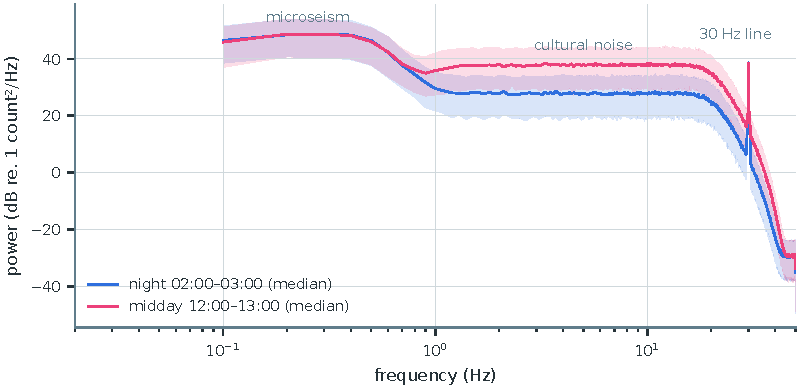
\includegraphics[width=\linewidth]{theory-psd-summary}
\caption{Noise spectrum of the demo EHZ channel for 02:00--03:00 (blue) and 12:00--13:00 (pink): median and
10th--90th percentile band, from the application's \code{spectrogram} and \code{psd\_summary}. Cultural noise above
1~Hz is clearly stronger at midday.}\label{fig:psd}
\end{figure}

\section{Relation to the McNamara--Buland PPSD}
The standard tool for describing the noise of a seismic station is the \emph{probabilistic power spectral density}
(PPSD) of \textcite{mcnamara2004}. Its recipe is: cut the data into one-hour segments; estimate a PSD for each with
Welch's method, correct it for the instrument response; smooth it into narrow period bands; and accumulate, for every
period, a histogram of the resulting power levels. The histograms, together with the global new low-noise and
high-noise models of \textcite{peterson1993}, show at a glance how quiet and how variable a site is.

The noise spectrum of RS3D is a deliberately simplified relative of the PPSD, and the differences matter when the
two are compared.

\begin{table}[tbp]
\centering\small
\caption{RS3D noise spectrum versus the PPSD of McNamara and Buland (2004).}\label{tab:ppsd}
\begin{tabular}{@{}L{0.23\linewidth}L{0.35\linewidth}L{0.35\linewidth}@{}}
\toprule
 & PPSD & RS3D noise spectrum\\ \midrule
Segments & one-hour, overlapping & the spectrogram windows of the chosen range\\
Averaging inside a segment & Welch average of sub-segments & none: each window is one periodogram\\
Instrument response & removed & \textbf{not} removed (counts$^2$/Hz)\\
Frequency smoothing & narrow octave fractions & none (linear bins)\\
Summary & full histogram per period & 10th, 50th and 90th percentile\\
Reference models & NLNM and NHNM & none\\
\bottomrule
\end{tabular}
\end{table}

\begin{rs3dwarn}[Not comparable with the Peterson noise models]
Because the response is not removed, the RS3D curve is in counts$^2$/Hz, not in the acceleration units of the
Peterson models, and its shape includes the geophone's own roll-off below 4.5~Hz. It must be used for
\emph{relative} comparisons on the same instrument (day versus night, this week versus last week), not to rank a site
against published noise levels.
\end{rs3dwarn}

\section{What the curves tell you}
\begin{description}[leftmargin=2.2cm,style=nextline]
\item[Microseism, 0.1--0.3~Hz] ocean waves coupling to the sea floor; present everywhere, strongest in winter storms. A
  short-period geophone sees it faintly because its response falls steeply below 4.5~Hz.
\item[Above 1~Hz] cultural noise (traffic, machinery, people). It changes with the time of day and the day of the week;
  the difference between the two curves of \cref{fig:psd} is a direct measure of it.
\item[Narrow peaks] a single frequency that never changes: interference. The 30~Hz line of the demo data is an example.
\item[Roll-off near 50~Hz] the digitiser's anti-alias filter (Chapter~\ref{ch:data}); it is a property of the instrument,
  not of the ground.
\end{description}

\begin{rs3dapp}
\code{psd\_summary(freqs, power\_db)} in \file{core/spectro.py} returns $(f, P_{10}, P_{50}, P_{90})$ using
\code{numpy.percentile} on the decibel values, after dropping gap columns and the zero-frequency bin. The chart is
\code{psd\_options} in \file{app/charts.py}.
\end{rs3dapp}
